\documentclass[11pt]{report}

\author{Darren Hushak}
\title{CPRE 308 Lab 2 - Lab Section E}
\date{}

\usepackage{tikz}

\begin{document}
\maketitle
\section*{Summary}
This lab was a quick exploration into some of the lower kernel level functions of Linux and the working of processes, forking, and process ID's. Interesting points I learned include the fact that orphan processes may be picked up by init, and I now have a better understanding of how linux boots (starting with init, which looks at inittab and gradually starts more and more processes until the OS is fully booted). It was also quite interesting to see the processor switching from one process to another with context switches.

\newpage
\section*{3.1 - Process Table}

In this portion of the lab, we inspected two processes which run for two minutes apiece. We were to run two of them, figure out the process ID and the parent process ID. Then we were to run them again and determine what changed.

\begin{verbatim}
./processTree &
\end{verbatim}

Output:
\begin{verbatim}
Process ID is: 1482
Parent process ID is: 30444
\end{verbatim}

\begin{verbatim}
./processTree &
\end{verbatim}

Output:
\begin{verbatim}
Process ID is: 1483
Parent process ID is: 30444
\end{verbatim}

\begin{verbatim}
ps -l
\end{verbatim}
\begin{itemize}
\item PS Output:
\end{itemize}
\begin{verbatim}
F S   UID   PID  PPID  C PRI  NI ADDR SZ WCHAN  TTY          TIME CMD
0 S 42706  1482 30444  0  80   0 -   981 hrtime pts/22   00:00:00 processTree
0 S 42706  1483 30444  0  80   0 -   981 hrtime pts/22   00:00:00 processTree
0 R 42706  1716 30444  0  80   0 - 27035 -      pts/22   00:00:00 ps
0 S 42706 30444 30443  0  80   0 - 28173 wait   pts/22   00:00:00 bash
\end{verbatim}

\begin{itemize}
\item Process Name :\begin{verbatim}processTree\end{verbatim}

\item Process State: S, which stands for "Sleeping"

\item PID: 1482 and 1483

\item PPID: 30444

\begin{verbatim} top -p 30444 \end{verbatim}

Output:
\begin{verbatim} 30444 dnhushak  20   0  110m 2072 1568 S  0.0  0.0   0:00.14 bash  \end{verbatim}

Therefore, the name of processTree's parent process is bash. Bash is a command language interpreter. Essentially what's happening is the ./processTree statement acted as an argument through stdin into bash. Bash interpreted that as a command, which was to run the compiled file with that name.

\end{itemize}

Repeat Process:

\begin{verbatim}
./processTree &
\end{verbatim}

Output:
\begin{verbatim}
Process ID is: 2761
Parent process ID is: 30444
\end{verbatim}

\begin{verbatim}
./processTree &
\end{verbatim}

Output:
\begin{verbatim}
Process ID is: 2762
Parent process ID is: 30444
\end{verbatim}

\begin{verbatim}
ps -l
\end{verbatim}

Output:

\begin{verbatim}
F S   UID   PID  PPID  C PRI  NI ADDR SZ WCHAN  TTY          TIME CMD
0 S 42706  2761 30444  0  80   0 -   981 hrtime pts/22   00:00:00 processTree
0 S 42706  2762 30444  0  80   0 -   981 hrtime pts/22   00:00:00 processTree
0 R 42706  2766 30444  0  80   0 - 27034 -      pts/22   00:00:00 ps
0 S 42706 30444 30443  0  80   0 - 28173 wait   pts/22   00:00:00 bash
\end{verbatim}
\pagebreak

\section*{3.2 - Fork()}
This section was an inspection of how forked processes actually execute, and how they relate to their parents. We were to run the fork program and see how their process ID's and parent PID's came out.

\begin{verbatim}
./fork1
\end{verbatim}

Output:

\begin{verbatim}
Process 6715’s parent process ID is 30444
Process 6717’s parent process ID is 6715
Process 6716’s parent process ID is 6715
Process 6718’s parent process ID is 6716
\end{verbatim}

Process Tree:
\\
\begin{center}
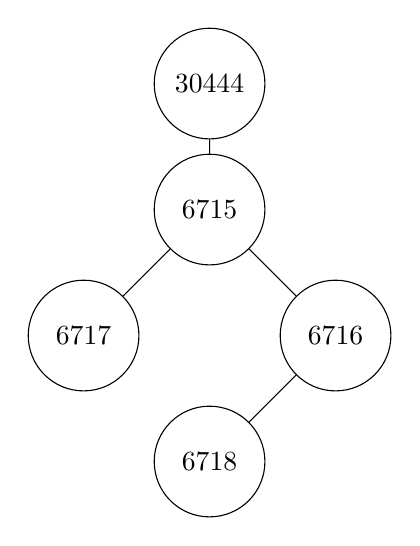
\begin{tikzpicture}
  [scale=.8,auto=left,every node/.style={circle, minimum width=40pt, draw}]
  \node (n1) at (5,6) {30444};
  \node (n2) at (5,4)  {6715};
  \node (n3) at (3,2)  {6717};
  \node (n4) at (7,2)  {6716};
  \node (n5) at (5,0)  {6718};

  \foreach \from/\to in {n1/n2,n2/n3,n2/n4,n4/n5}
    \draw (\from) -- (\to);

\end{tikzpicture}
\end{center}
An explanation:
\\
The initial process (fork1, with a PID of 6715) starts, gets to the first fork(), and generates a new process, with PID 6716. 6715 gets to its next fork() before 6716 is fully initialized, and then creates a new process with PID 6717. Since 17 was created after the second fork, it runs to completion without forking any more processes. Process 6716 is now finally initialized, and still has one fork left (since it was forked from the first fork in 6715). This fork then generates process 6718.
\\
Now, remove the sleep(2) command:

\begin{verbatim}
./fork1
\end{verbatim}

Output:

\begin{verbatim}
Process 13966’s parent process ID is 30444
Process 13967’s parent process ID is 1
Process 13968’s parent process ID is 1
Process 13969’s parent process ID is 1
\end{verbatim}

In this instance, the initial process (PID 13966) executes and exits before any of the forked processes are fully initialized. Because their parent process no longer exists, they are then 'adopted' by PID 1, which is init.


\section*{3.3 - Fork() Continued}
This section had an expansion of Fork in which we utilize the return value of fork to determine whether or not a forked process is a child or parent.

To complete the code, the conditional statement that the if is checking needs to be changed to:
\begin{verbatim}
if (ret == 0) {
\end{verbatim}

This checks the returned value of the fork. The fork returns 0 for child, which is what we are checking to see in the if statement.

\begin{verbatim}
./fork2
\end{verbatim}

Output:
\begin{verbatim}
The parent process ID is 16203
The parent’s parent process ID is 30444
The child process ID is 16204
The child’s parent process ID is 16203
\end{verbatim}

\newpage
\section*{3.4 - Time Slicing}
This section we inspected Time Slicing by running a program that forks itself, and runs in parallel with its forked process. We were to inspect the output to see how the two processes run simultaneously.

\begin{verbatim}
./timeSlice
\end{verbatim}

Output (partial):

\begin{verbatim}
Parent: 2604
Parent: 2605
Child: 0
Child: 1
Child: 2
...
Child: 2821
Child: 2822
ChParent: 2606
Parent: 2607
Parent: 2608
...
Parent: 5125
Parent: ild: 2823
Child: 2824
\end{verbatim}

What we are witnessing here are context switches. The timeSlice process forked itself, and then runs through a very long iteration. Its forked process will also run through that same iteration, once it is initialized. Because the iteration is very long, the kernel scheduler will switch back and forth between the parent and child processes numerous times before both have finished the iteration. When we see the counter switch from parent to child in stdout, that is indicative of the kernel scheduler having given the child process processor time.

Note also the point at which "ChParent: 2606" occurs. This isn't any sort of error or bug, it's just simply a context switch right in the middle of child's printf statement. Later on in the code, the remaning "ild: 2823" with newline shows up again when the context switches back to the child.

\newpage
\section*{3.5 - Wait()}
Here we ran a program that included the wait() command, which simply waits until all children processes have completed.

\begin{verbatim}
./waitSync
\end{verbatim}

Output(Partial):
\begin{verbatim}
Child starts
Child: 0
Child: 1
Child: 2
...
Child: 499999
Child ends
Parent starts
Parent: 0
Parent: 1
\end{verbatim}

Here the code is rather similar between waitSync and timeSlice, but the effect is very different. In waitSync, the extra wait() command before the iteration tells the parent process to wait until the child process has exited or been killed before advancing further. This is why we see the child to completion without any context switches.

\section*{3.6 - Kill()}
Here we inspected the kill() command, and tried to time the killing of a child process.

\begin{verbatim}
./killTest
\end{verbatim}

Output(Partial):
\begin{verbatim}
Parent sleeping
Child at count 1
...
Child at count 987
Child at count 988
Child has been killed. Waiting for it...
done.
\end{verbatim}


In this program, the child process has a while(1) (infinite) loop, and continually prints out a counted value. In this case, it's counting once every 1/100 of a second.

The parent process doesn't enter the loop, however, and sleeps after the fork for 10 seconds, then kills all of its children (oh the horror!). Because of this killing, the child process breaks out of the infinite loop by force of its parent (it's just not FAIR!).

Since the child is outputting every 1/100 of a second and the parent is to wait 10 seconds before killing its child (the world's a brutal place), the child should count to 1000 before dying. The output my program gave was close to 1000 before it was killed, which corroborates with my theory. The child doesn't fully reach the count because of the amount of time it takes for the context switch to take effect, so some time is lost between when the parent started waiting and the child process began.

\section*{3.7 - Execve()}
Here we run the code and examine the output. We were to determine when the print statment would occur, if it would.

\begin{verbatim}
./execfunction
\end{verbatim}
 Output:
 \begin{verbatim}
execFunction    fork1    fork2    killTest    mainReturn    Makefile  
processTree timeSlice    waitSync    zombieMaker.c    execFunction.c    
fork1.c    fork2.c  killTest.c  mainReturn.c  out       
processTree.c  timeSlice.c  waitSync.c
 \end{verbatim}
 
 Here execl() is calling /bin/ls, which simply runs another program, in this case "ls", which is why we see the current directory listing after running execl. The only way that the print statement could execute is if execl returned, which would only occur because of an error. Say execl was calling a non-existent program, that would return an error.
 
\newpage
\section*{3.8 - The return Value of Main()}

This section we ran a program a number of times and saw a string of random output numbers.

The output range seemd to be roughly 3 to 250 for both the child exit status and the terminate signal always seemed to be 15.
These values would be useful to determine if a child process was killed or if it ran to completion.



\newpage
\section*{3.9 - (Extra Credit) Zombie Processes}
A zombie process is a process that has completed its execution but has not exited, and is therefore still listed as a process on the process table.

The zombie program I wrote forked itself, and then checked whether or not it was the parent or child. If it was the child, it exited. If parent, it waited for 60 seconds and then returned.
\begin{verbatim}
#include <stdlib.h>
#include <sys/types.h>
#include <unistd.h>

int main ()
{
  pid_t childPID;

  childPID = fork ();
  //Check if child. If not, then sleep
  if (childPID > 0) {
    sleep (60);
  } 
  //If child, then exit
  else {
    exit (0);
  }
  return 0;
}
\end{verbatim}

To test, I ran the zombie maker in the background and then checked the process table:
\begin{verbatim}
./zombieMaker &
ps -l
\end{verbatim}


The output of ps gives:
\begin{verbatim}
F S   UID   PID  PPID  C PRI  NI ADDR SZ WCHAN  TTY          TIME CMD
0 S 42706 12076 30166  0  80   0 -   980 hrtime pts/27   00:00:00 zombieMaker
1 Z 42706 12077 12076  0  80   0 -     0 exit   pts/27   00:00:00 zombieMaker <defunct>
0 R 42706 12078 30166  0  80   0 - 27034 -      pts/27   00:00:00 ps
0 S 42706 30166 30095  0  80   0 - 28173 wait   pts/27   00:00:00 bash
\end{verbatim}
Here we can se the zombieMaker with PID of 12077 has a status of "Z" indicating Zombie.


\end{document}
